% \begin{figure*}[t]
% \centering
% 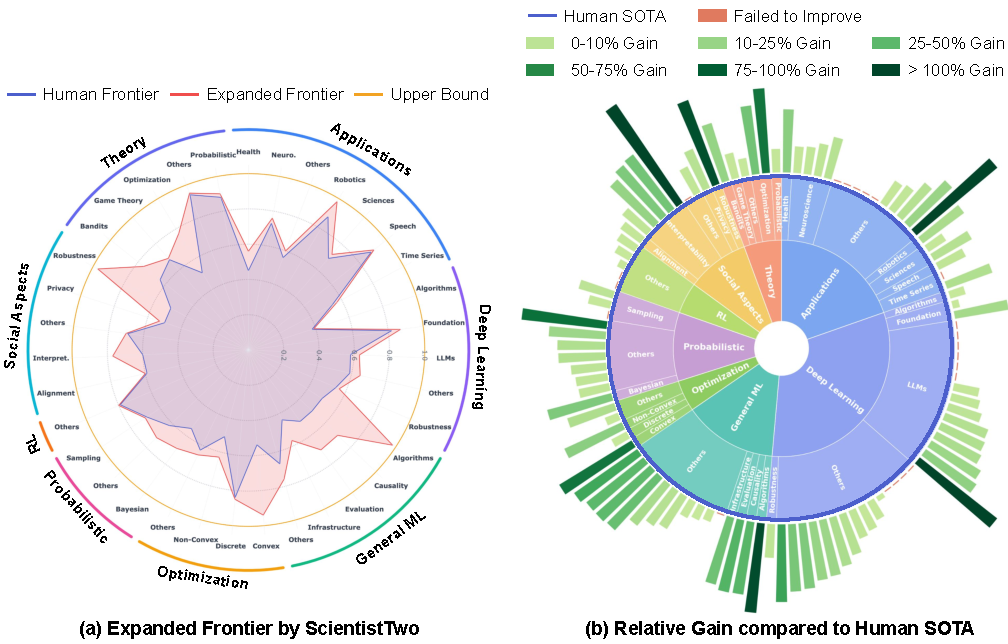
\includegraphics[width=\linewidth]{figures/sc2_new_fig2.pdf}
% \caption{\textbf{Problem setup.} \sname~automatically pushes the boundaries of human knowledge frontier by generating publication-quality papers and fully verified codebases, with resulting proposed novel methodologies consistently outperform human state-of-the-art baselines.}
% \label{fig:problem_setup}
% \end{figure*}
\begin{figure*}[t]
\centering
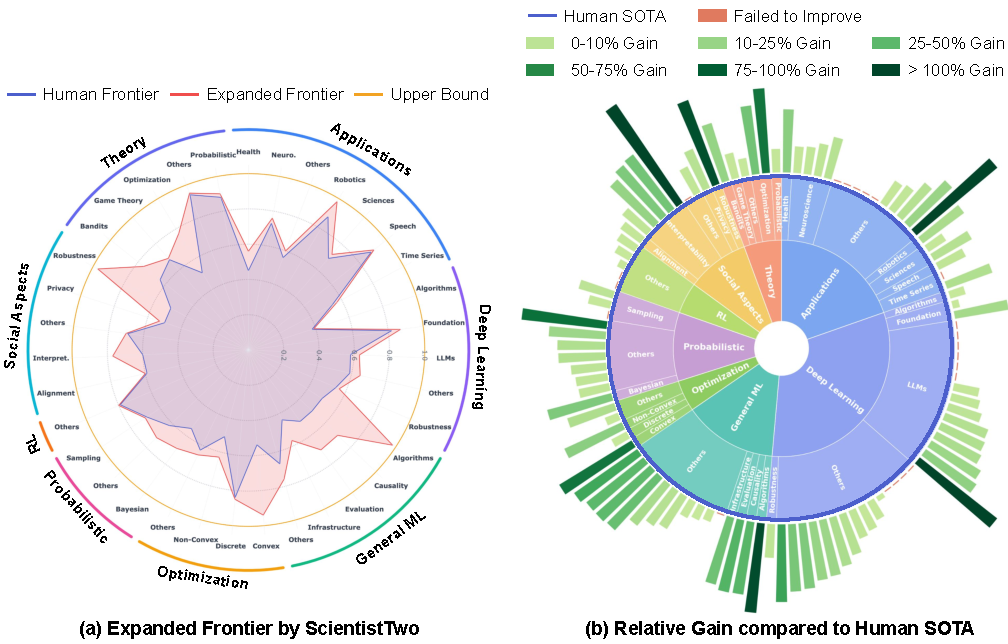
\includegraphics[width=\linewidth]{figures/sc2_new_fig2.pdf}
\caption{\textbf{Teaser.} \sname~pushes the frontier of human knowledge across diverse research domains (e.g., LLMs, robotics, neuroscience, speech, robustness, reinforcement learning, game theory, privacy, optimization, and time series) by generating publication-quality papers and fully verified codebases, with the resulting methodologies consistently outperforming human state-of-the-art baselines. Specifically, \sname~improves 86 out of 107 papers (an 80.4\% success rate) with an average relative improvement of 25.2\% over human state-of-the-art methods. Furthermore, papers generated by \sname~surpass the average scores of accepted papers at ICLR 2026 and NeurIPS 2025 under the Stanford Agentic Reviewer, demonstrating its capability to produce manuscripts that reach the empirical acceptance standards of top-tier AI venues.}
\label{fig:problem_setup}
\end{figure*}
\section{Introduction}

\begin{figure}[t]
  \centering
  \setlength{\tabcolsep}{0pt} 
  \renewcommand{\arraystretch}{0}
  \resizebox{\textwidth}{!}{
  \begin{tabular}{|c|c|c|c|c|}
  \hline
    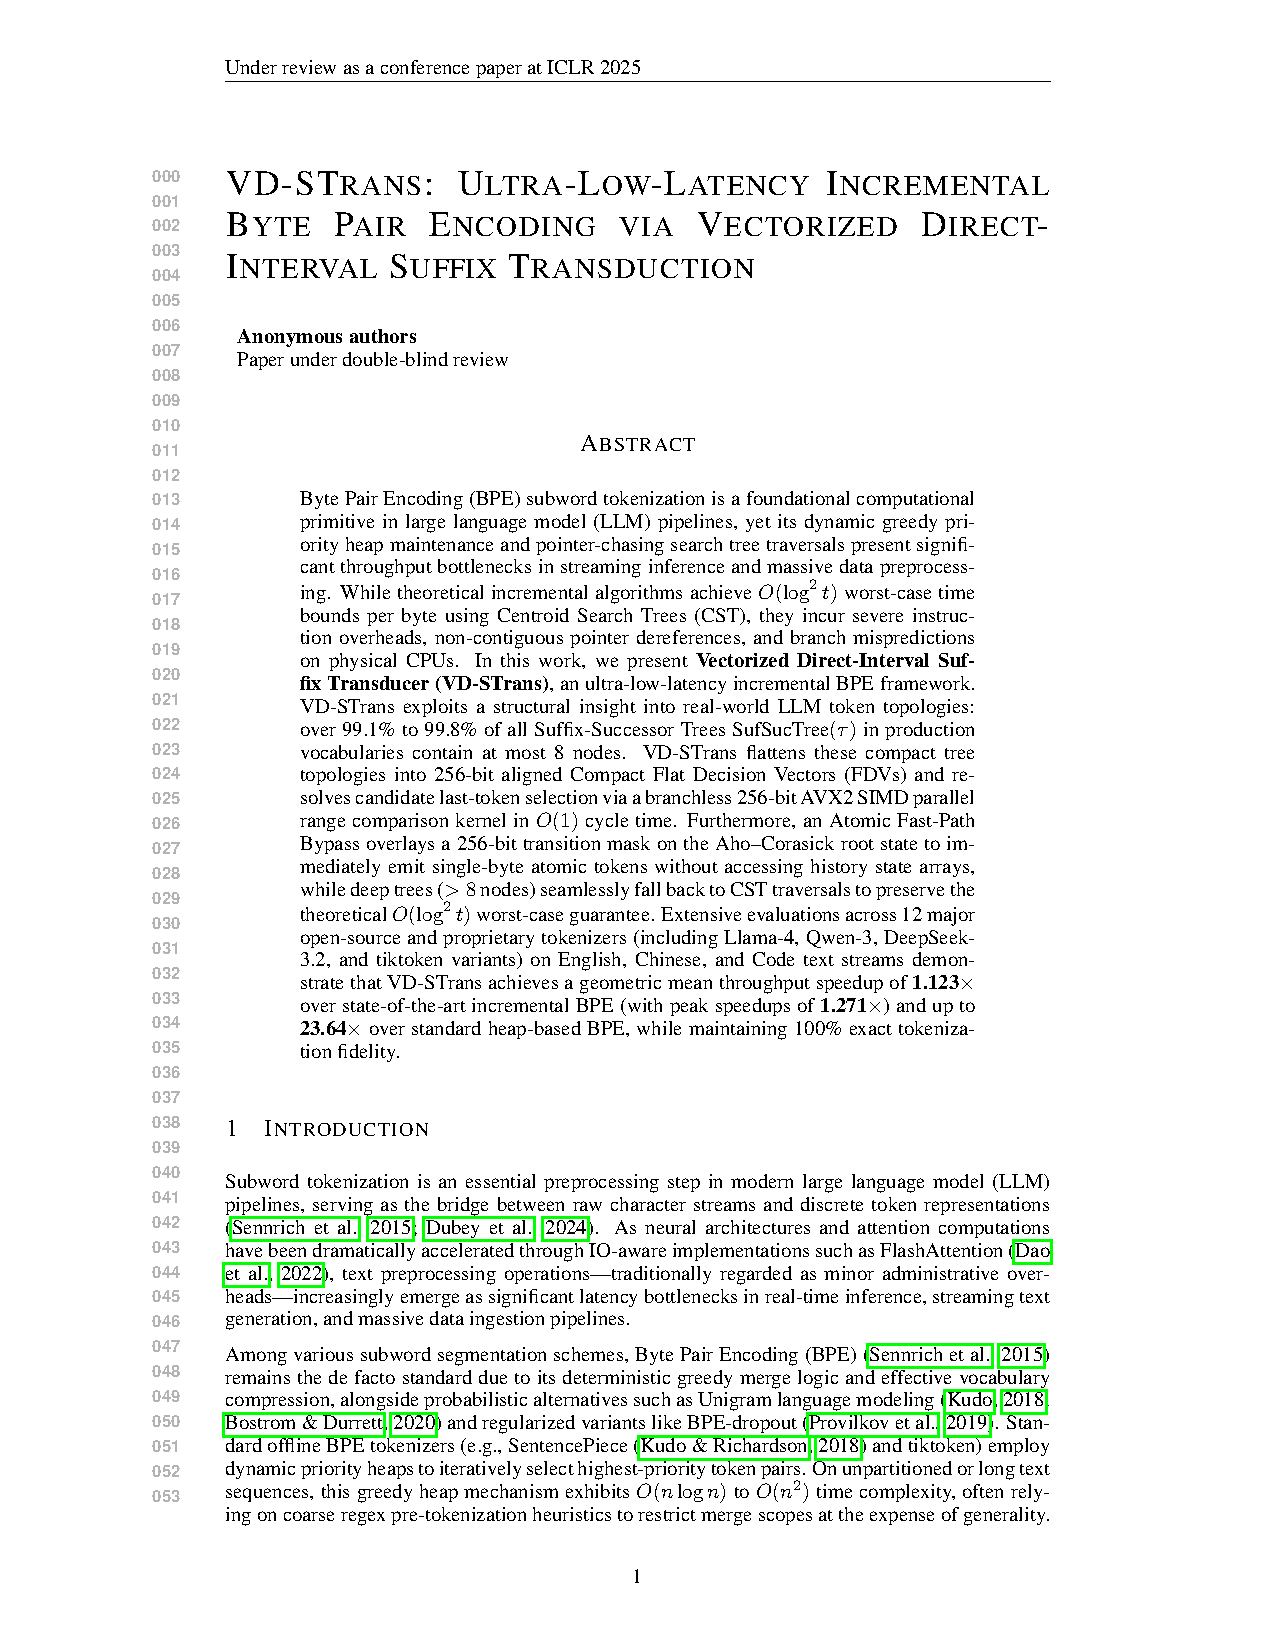
\includegraphics[width=0.2\textwidth]{figures/fig1_pdfs/page0.pdf} &
    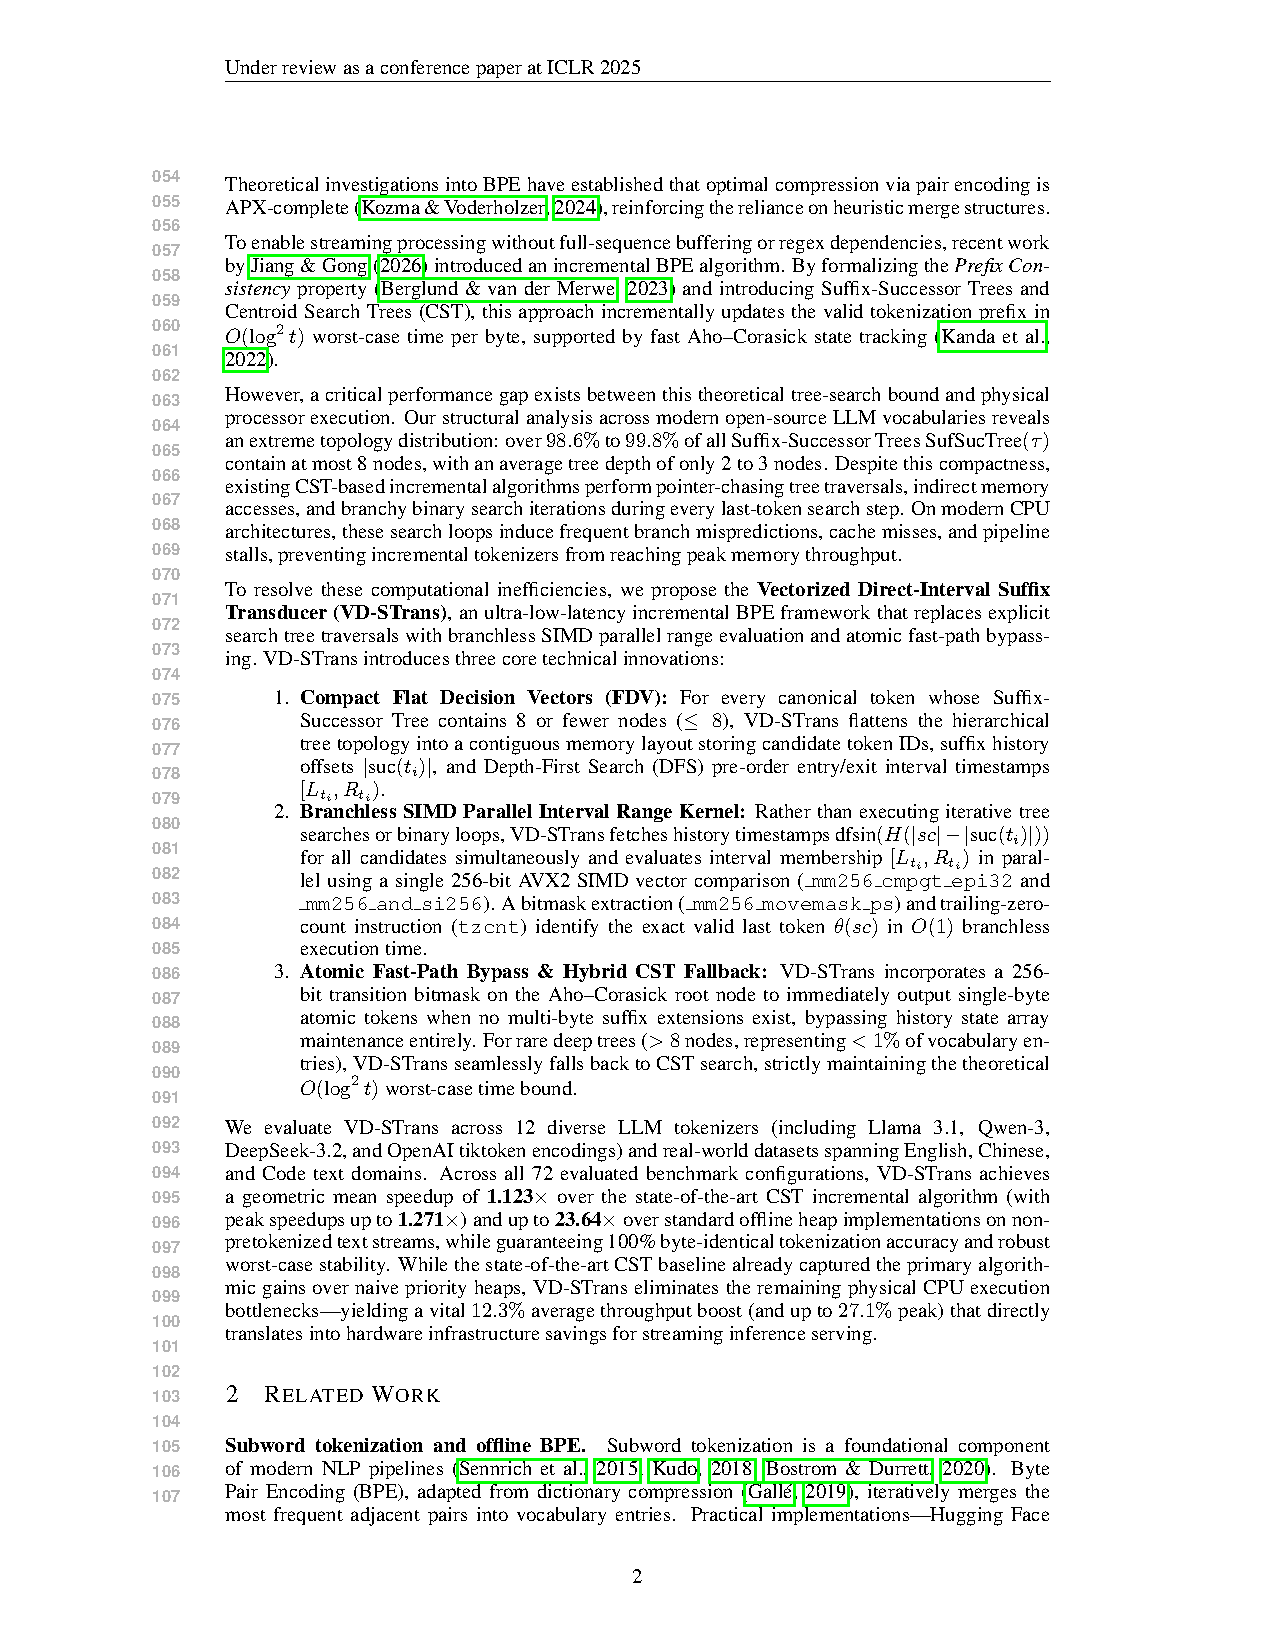
\includegraphics[width=0.2\textwidth]{figures/fig1_pdfs/page1.pdf} &
    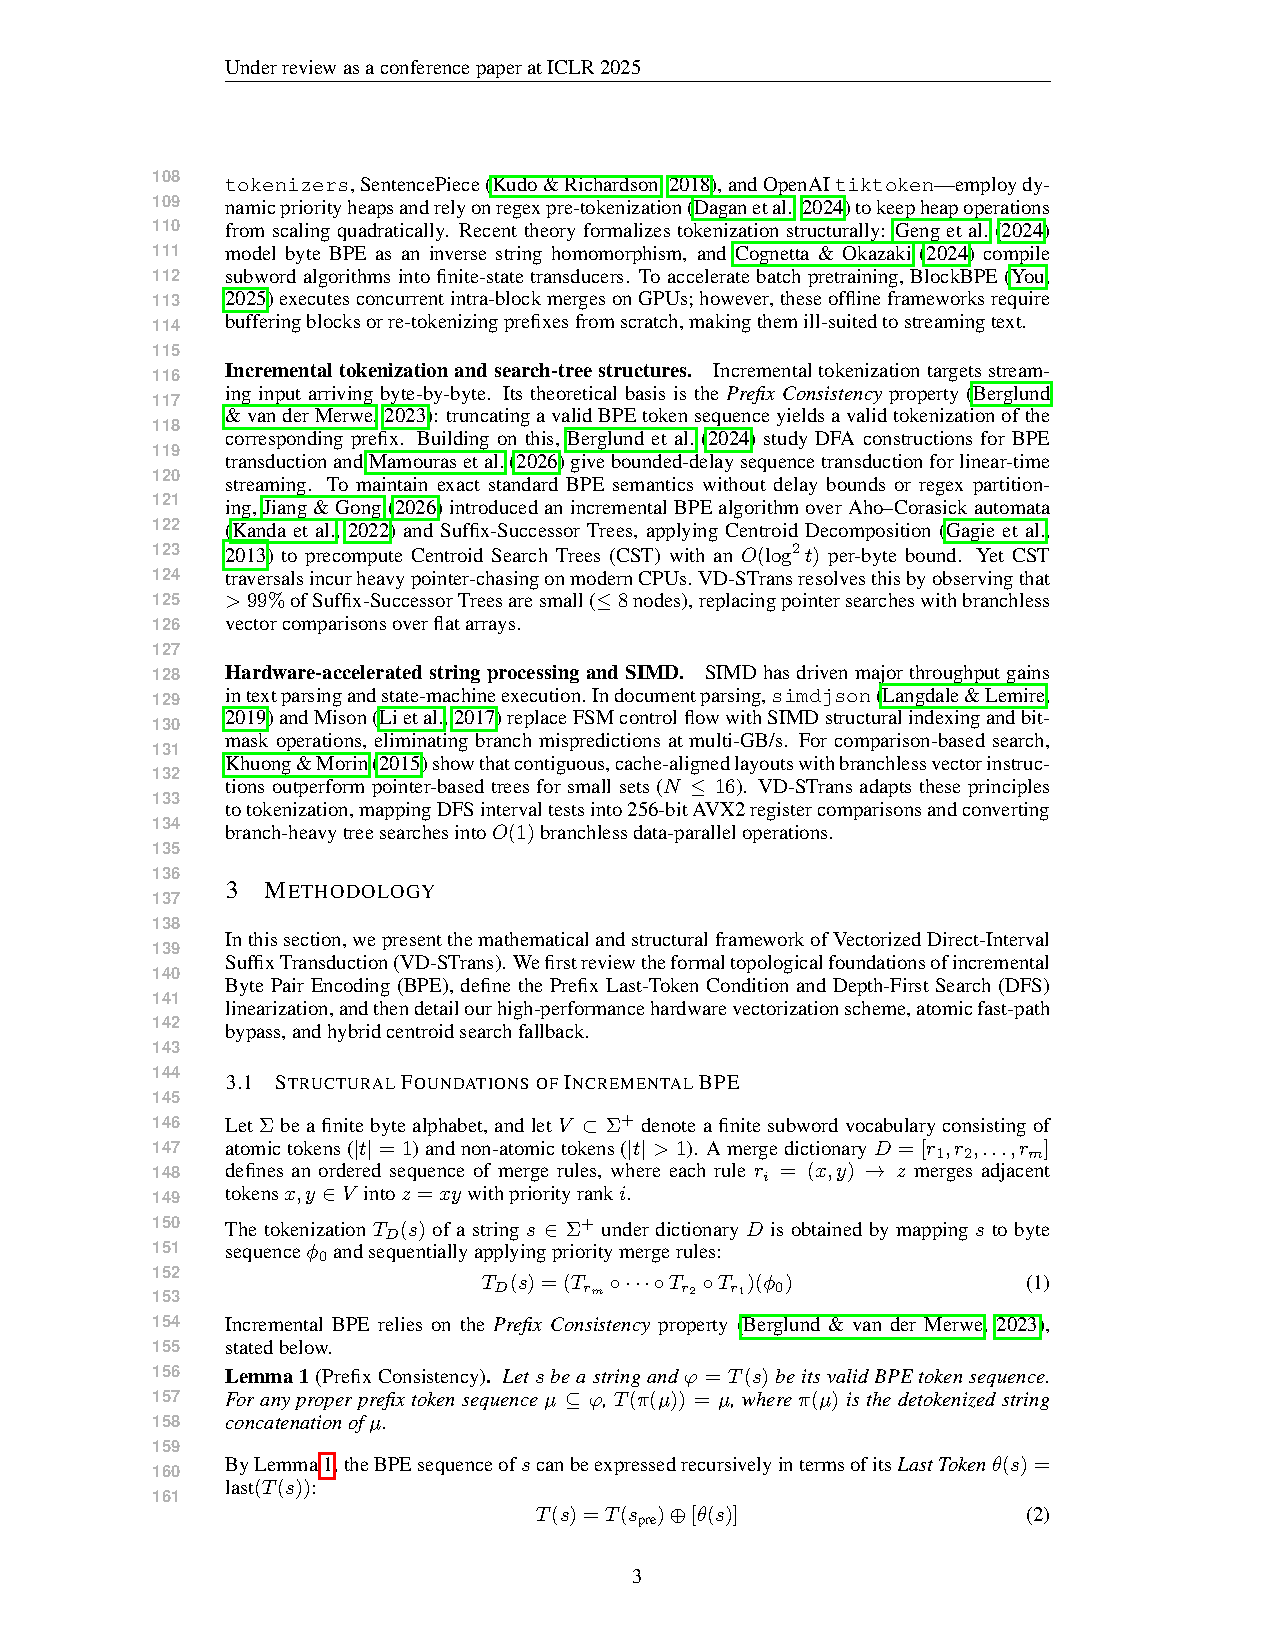
\includegraphics[width=0.2\textwidth]{figures/fig1_pdfs/page2.pdf} &
    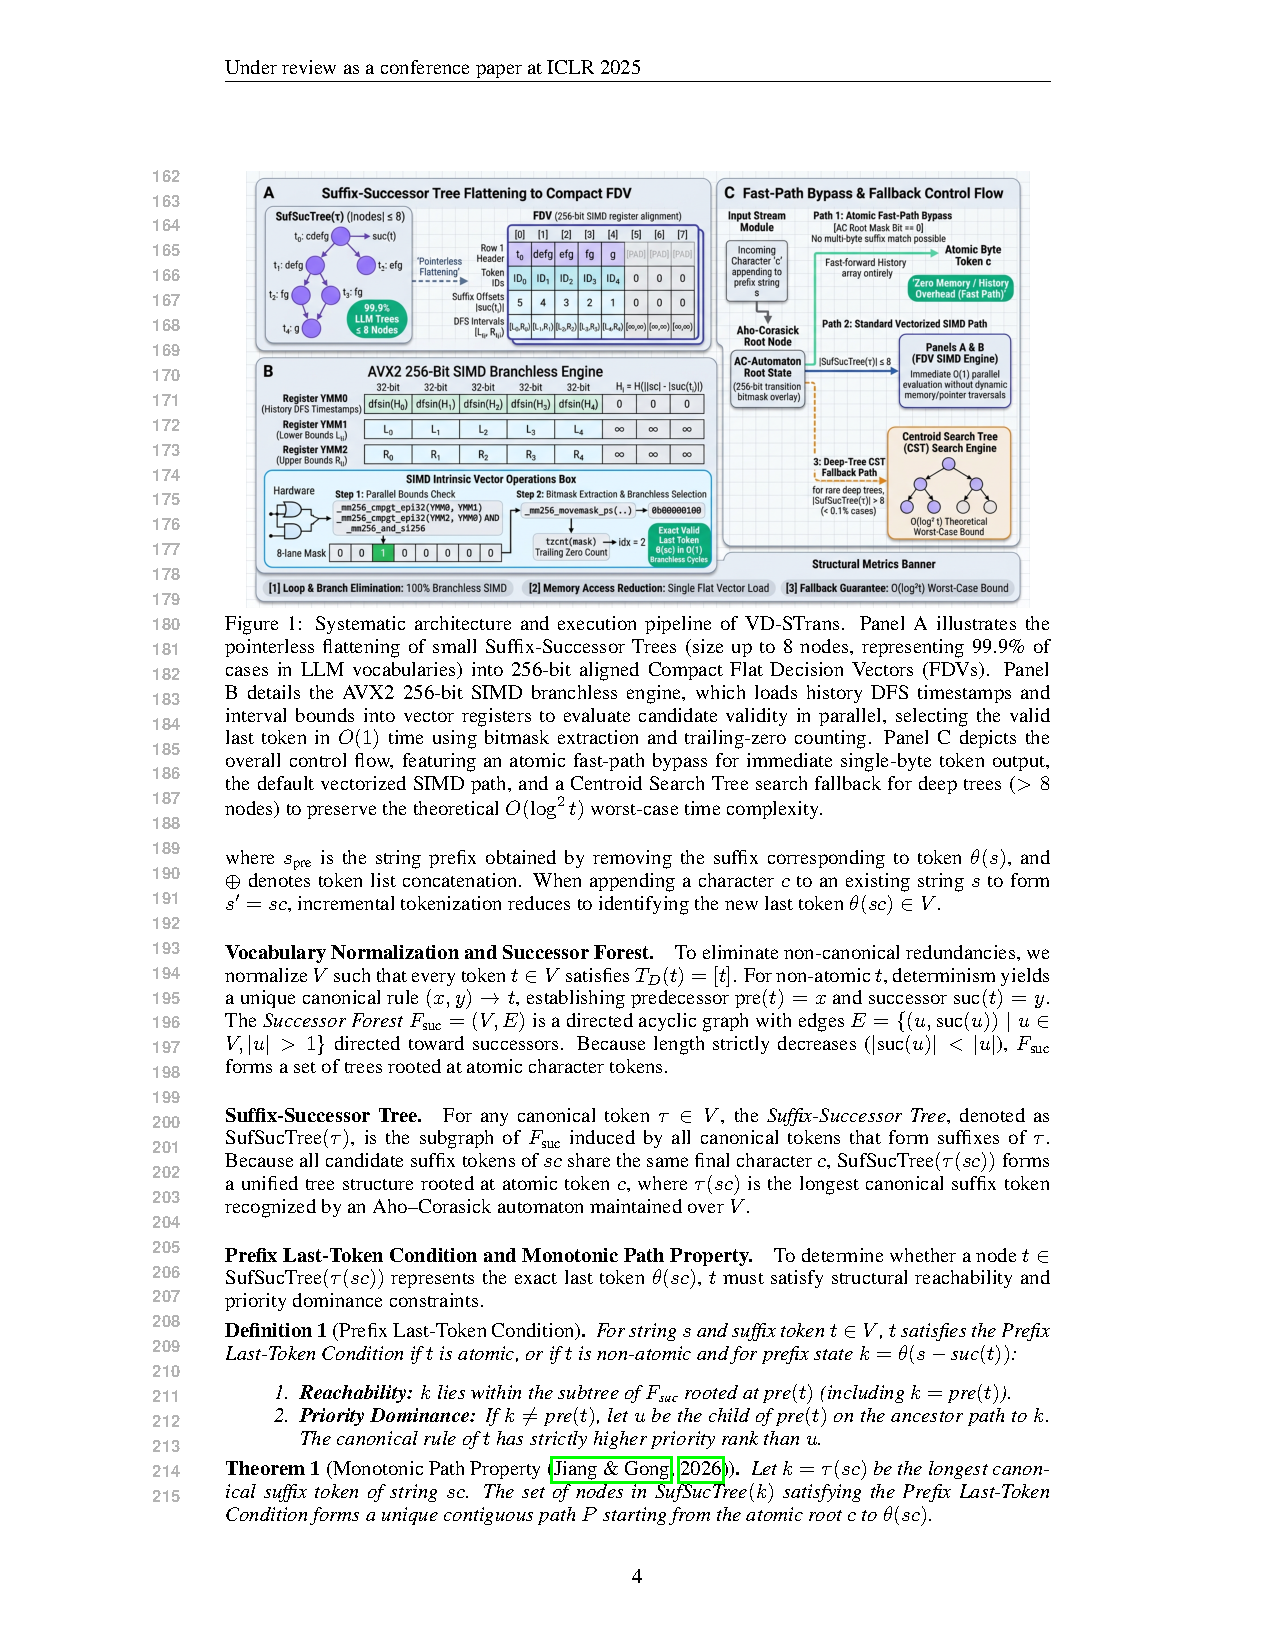
\includegraphics[width=0.2\textwidth]{figures/fig1_pdfs/page3.pdf} &
    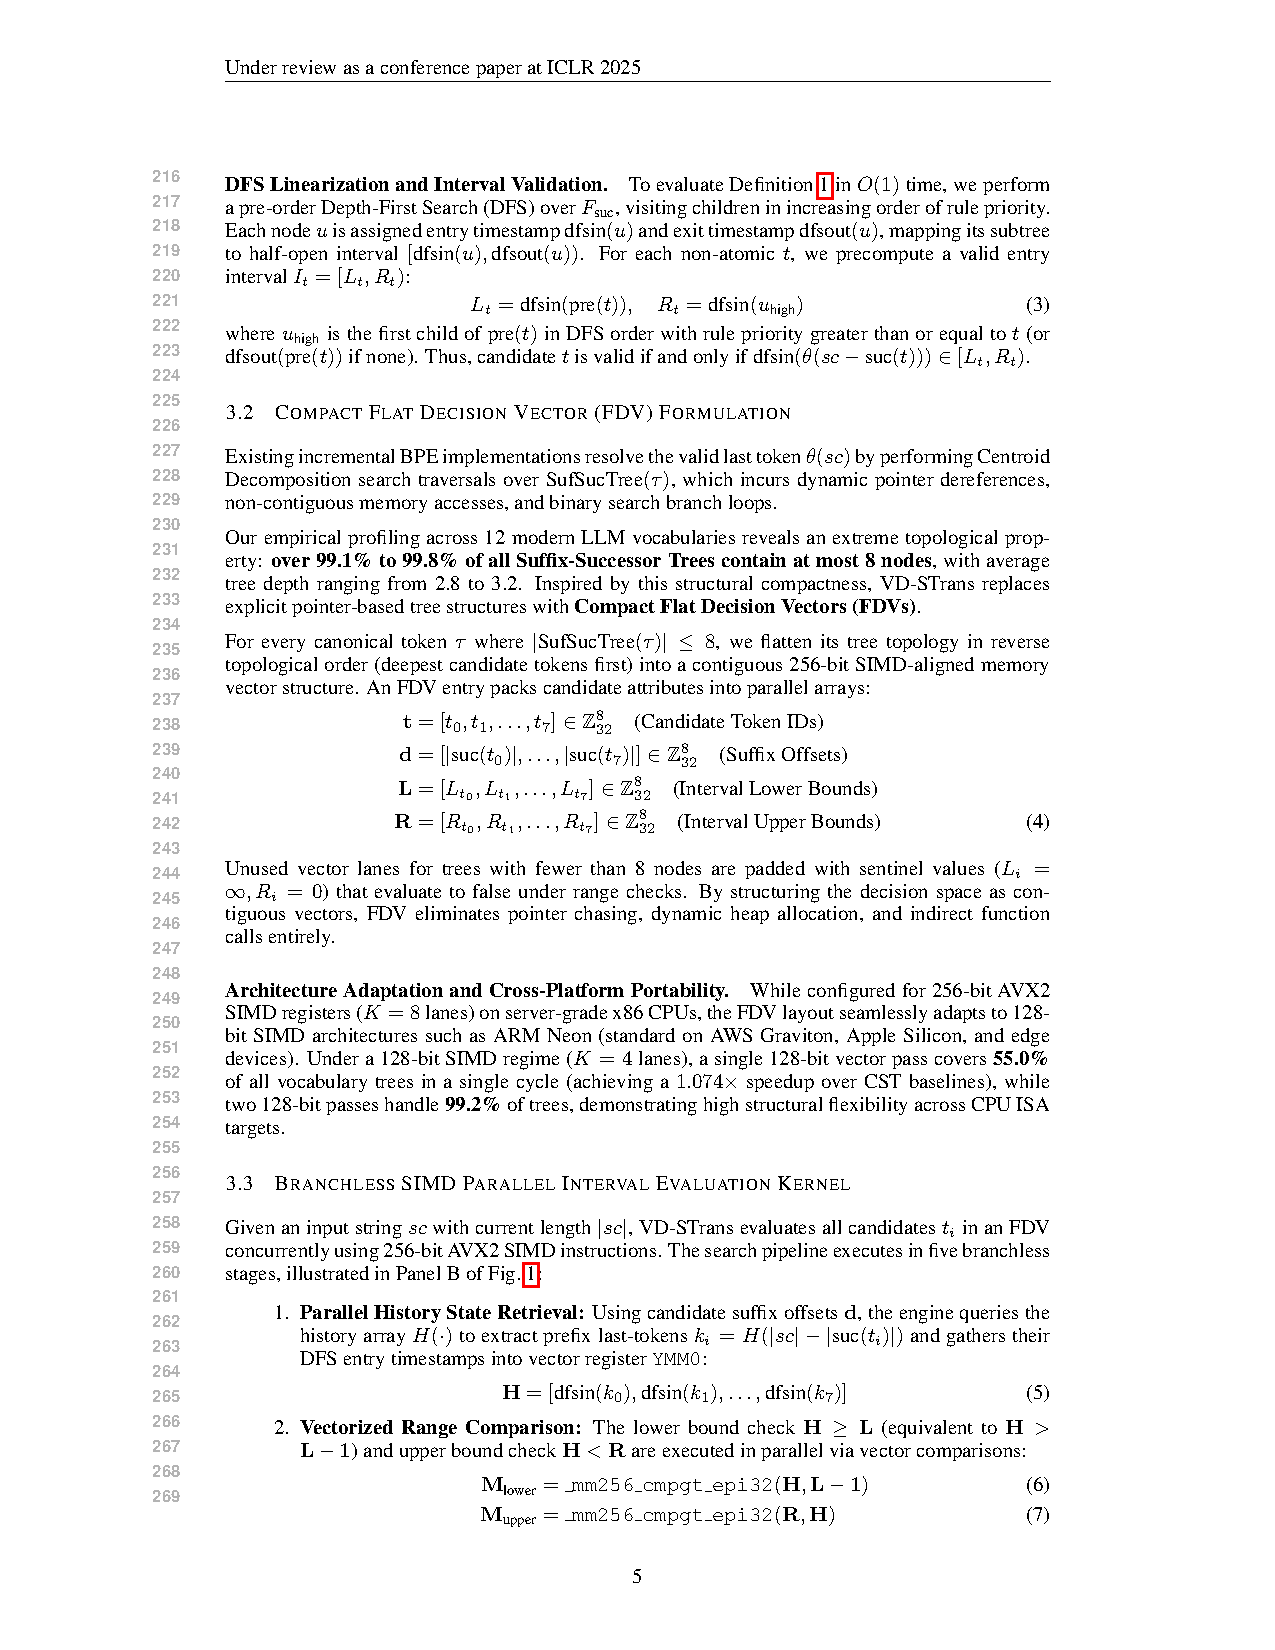
\includegraphics[width=0.2\textwidth]{figures/fig1_pdfs/page4.pdf} \\
    \hline
    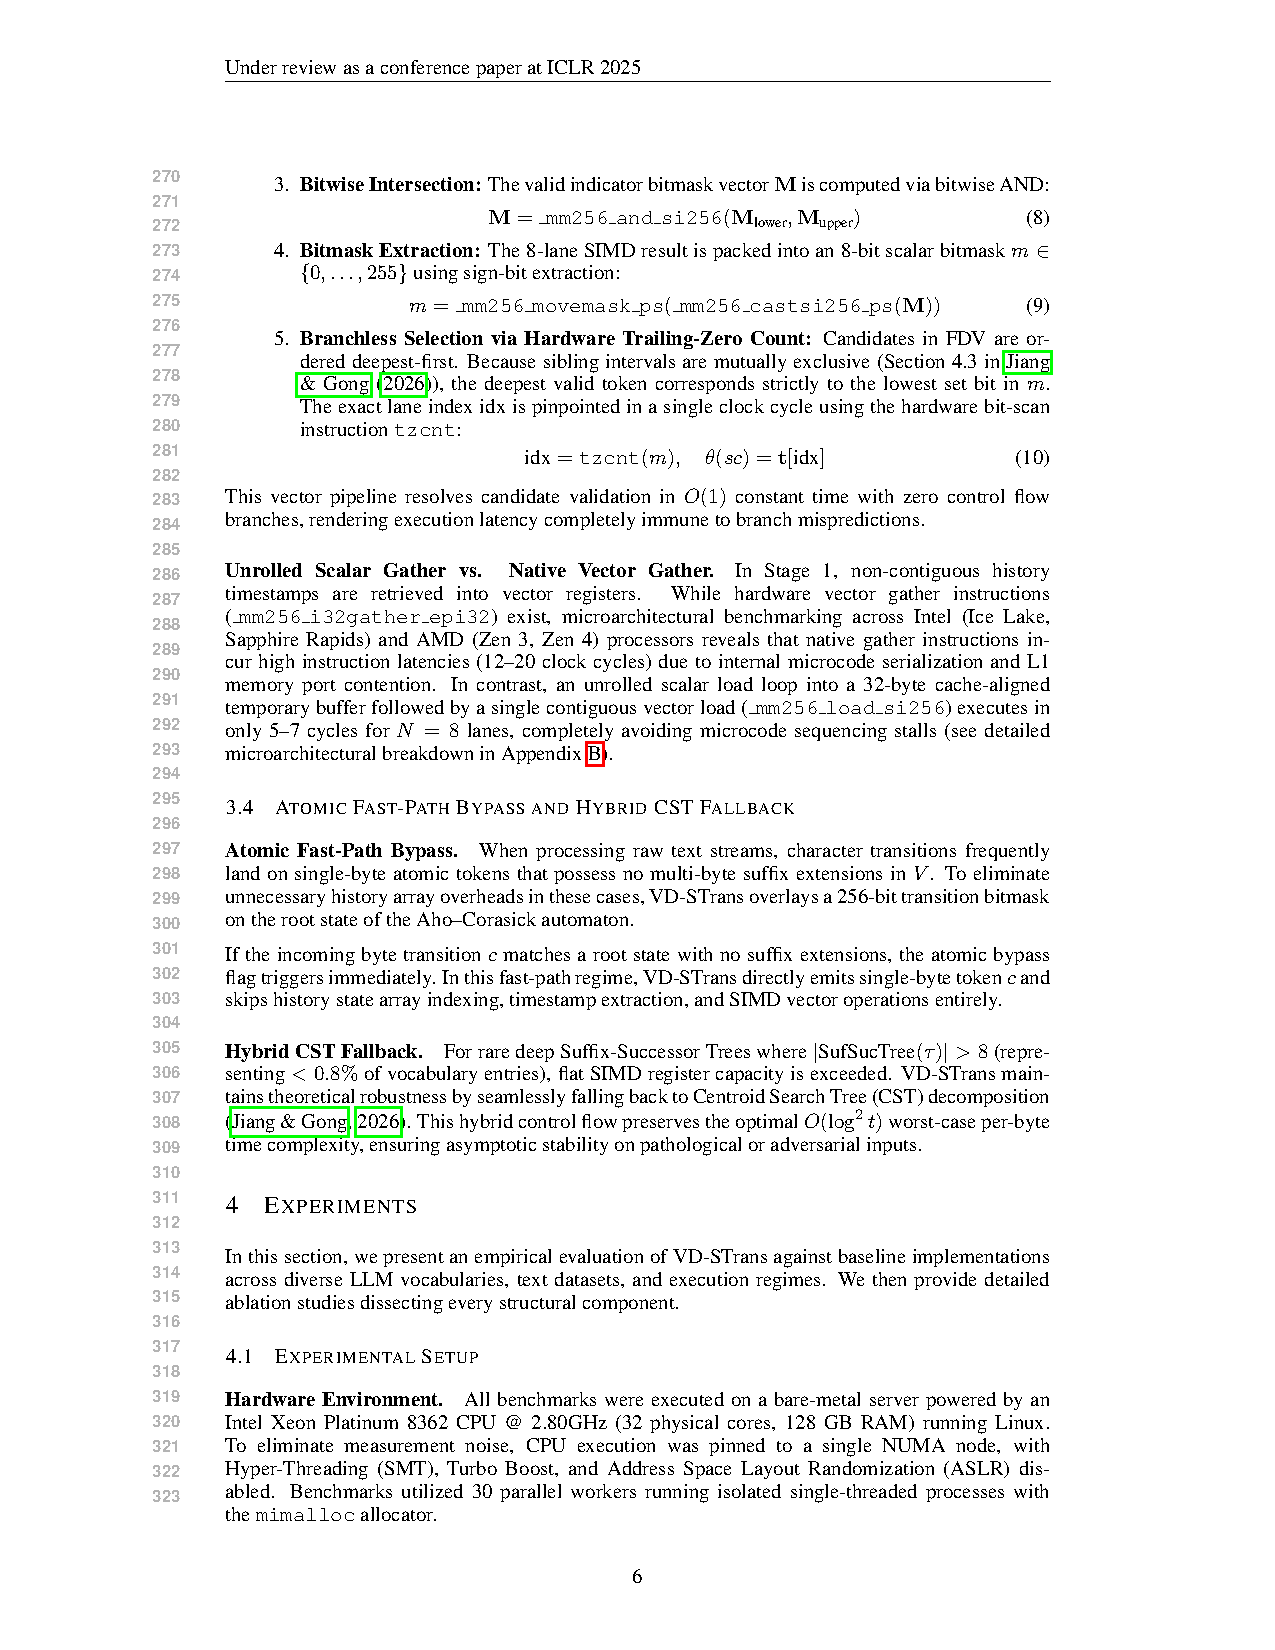
\includegraphics[width=0.2\textwidth]{figures/fig1_pdfs/page5.pdf} &
    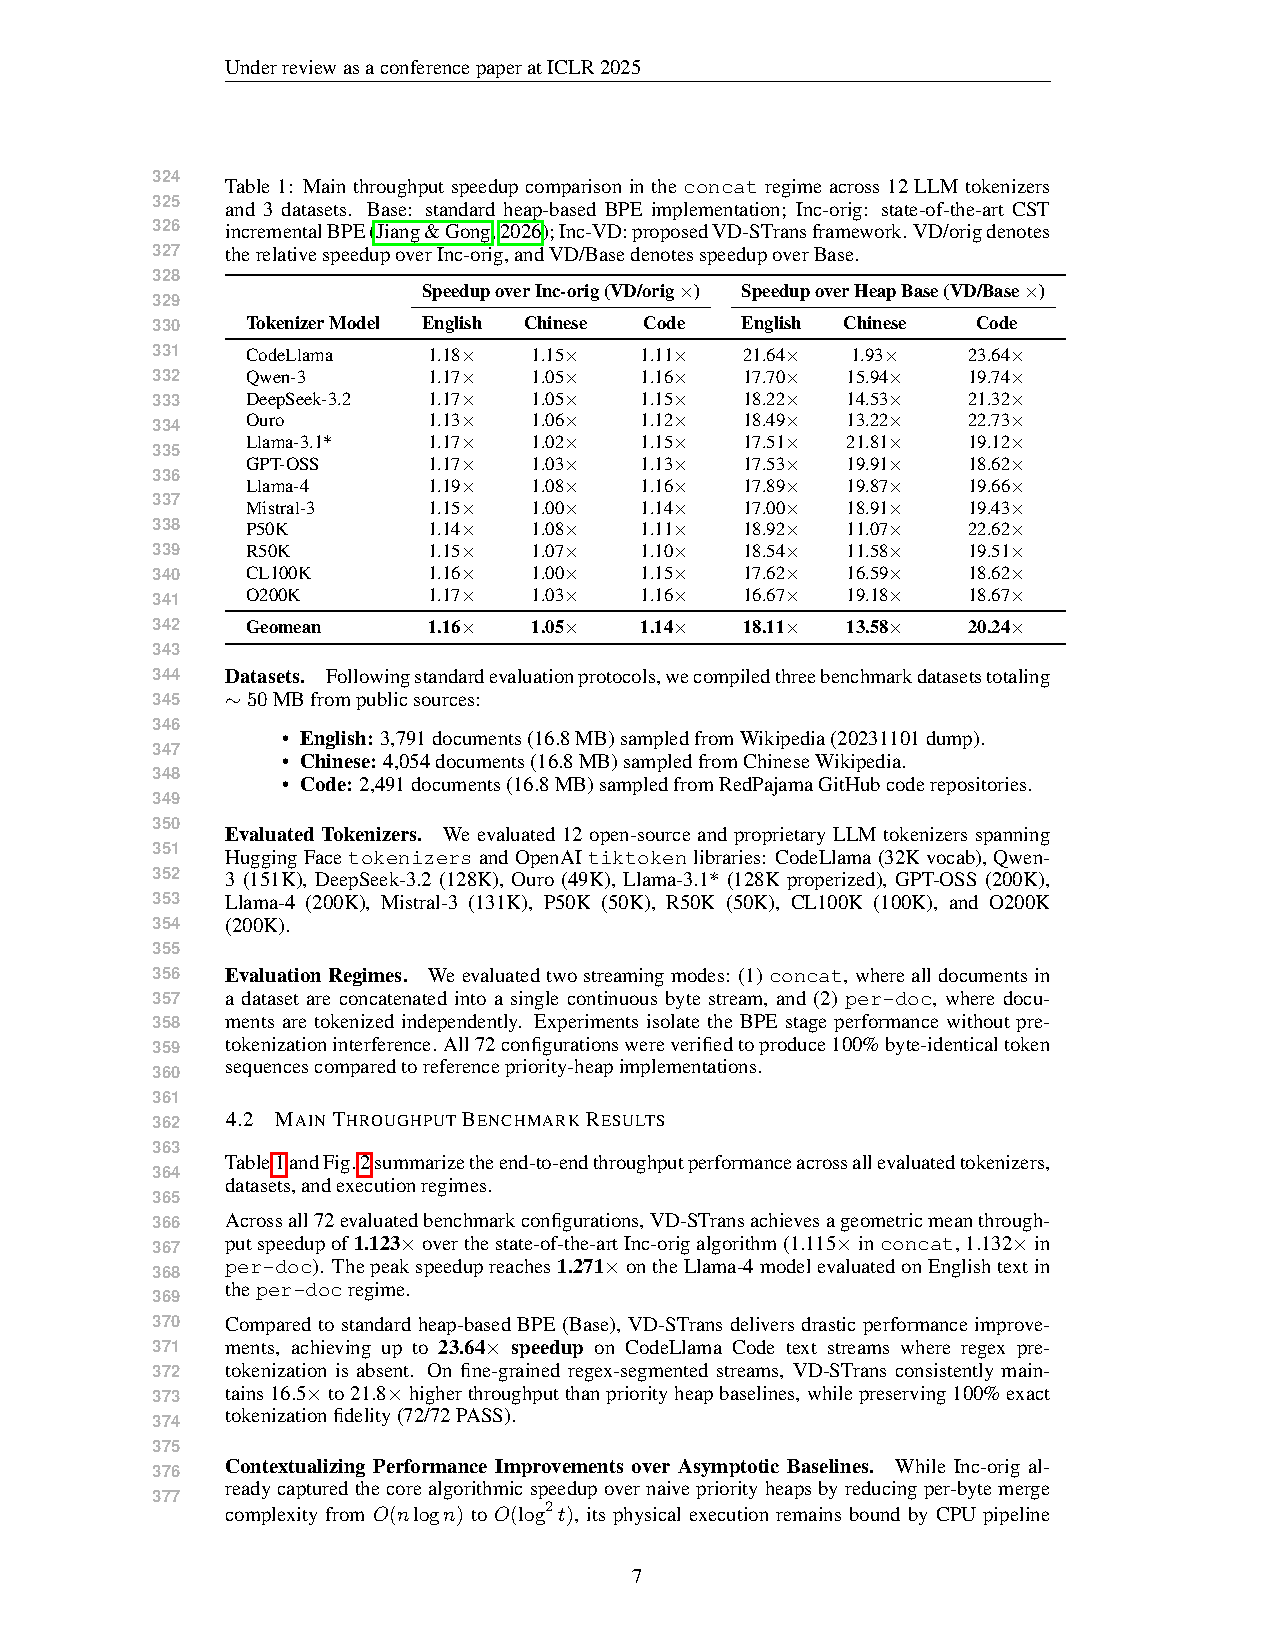
\includegraphics[width=0.2\textwidth]{figures/fig1_pdfs/page6.pdf} &
    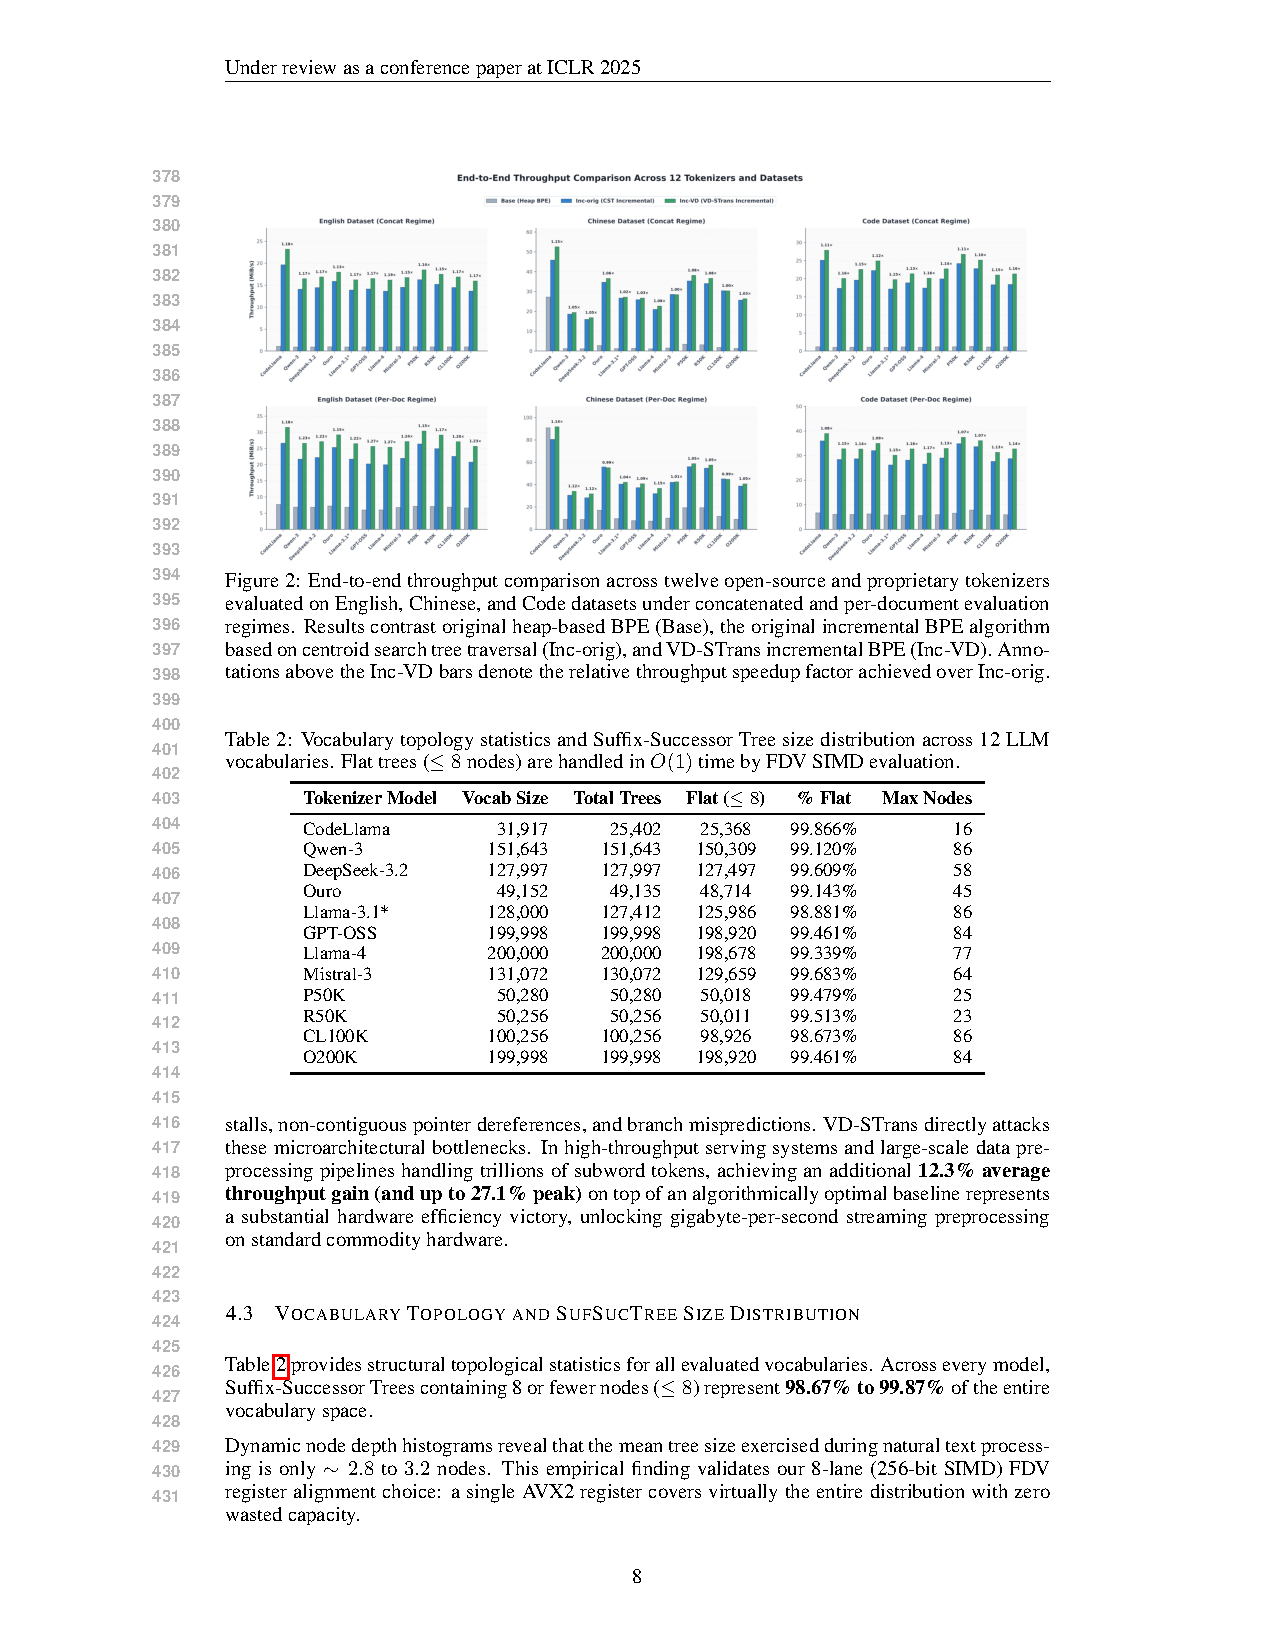
\includegraphics[width=0.2\textwidth]{figures/fig1_pdfs/page7.pdf} &
    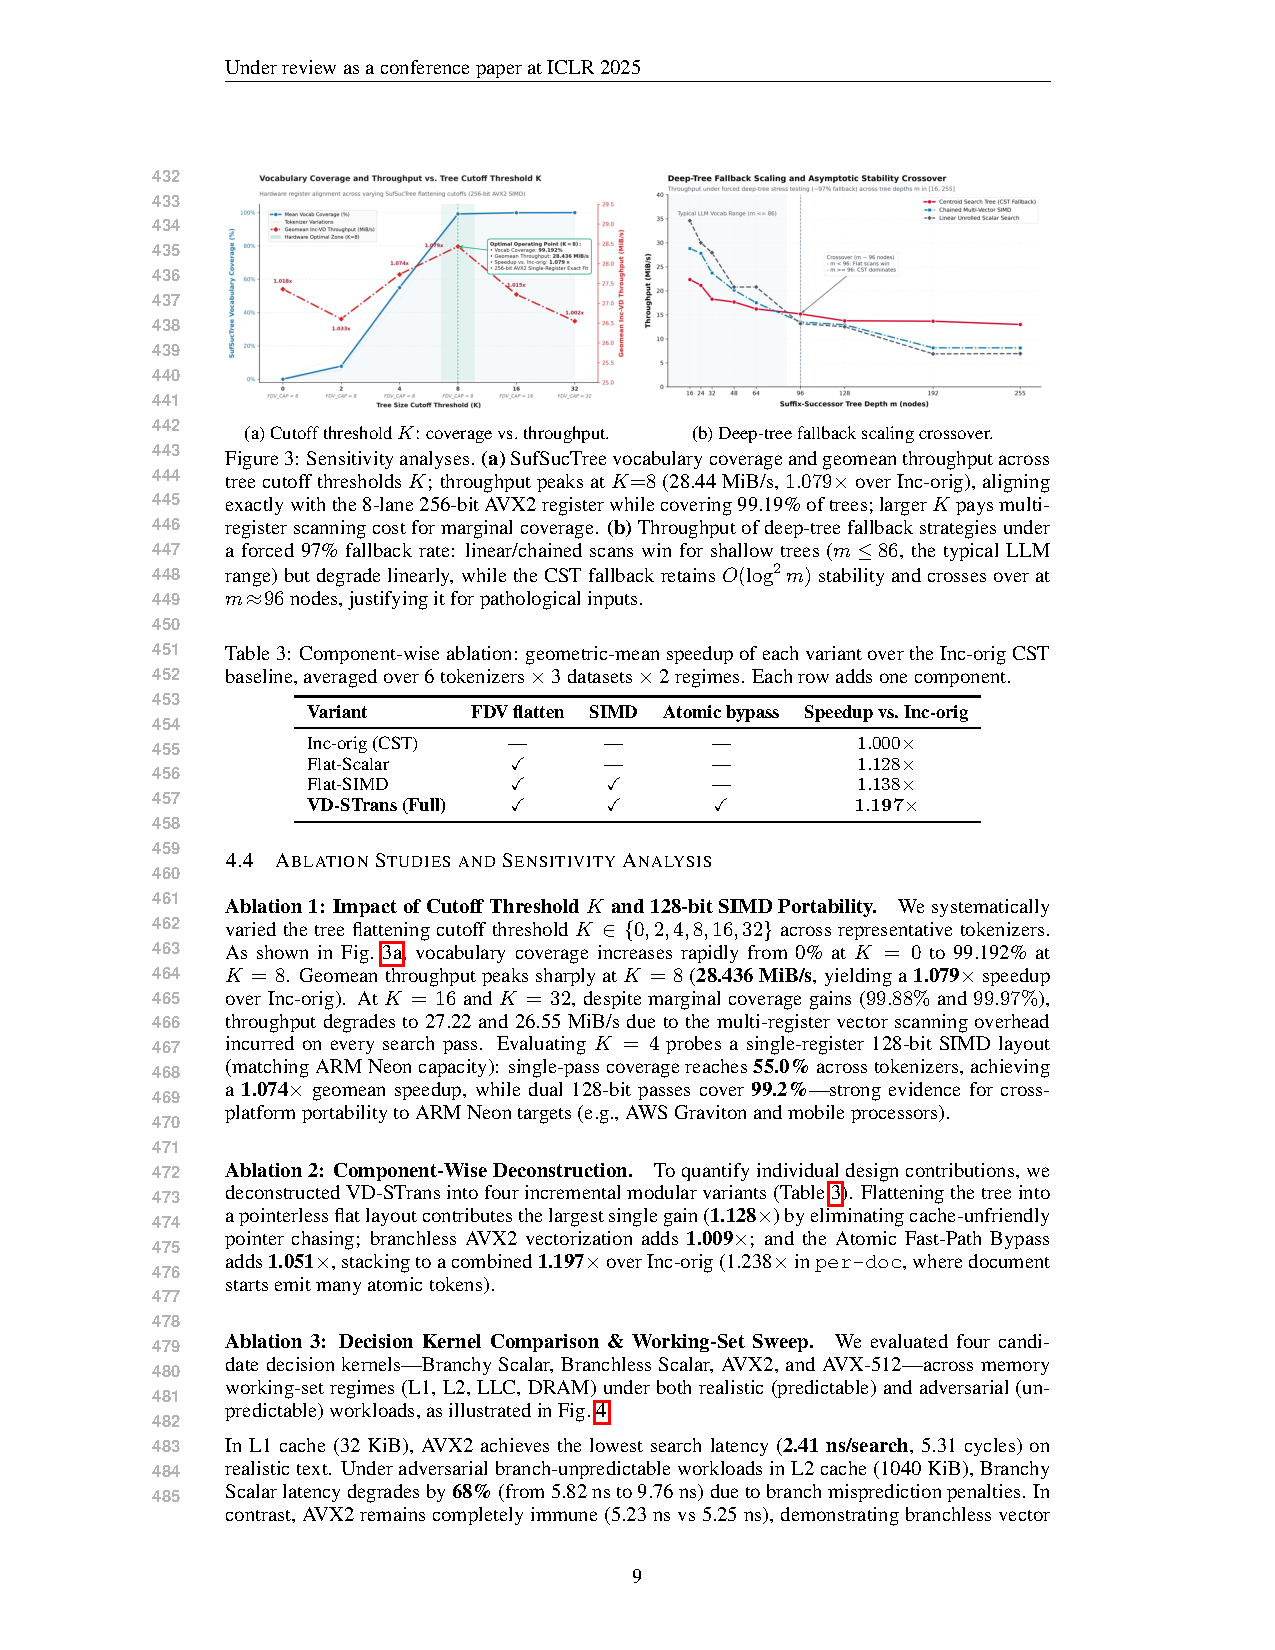
\includegraphics[width=0.2\textwidth]{figures/fig1_pdfs/page8.pdf} &
    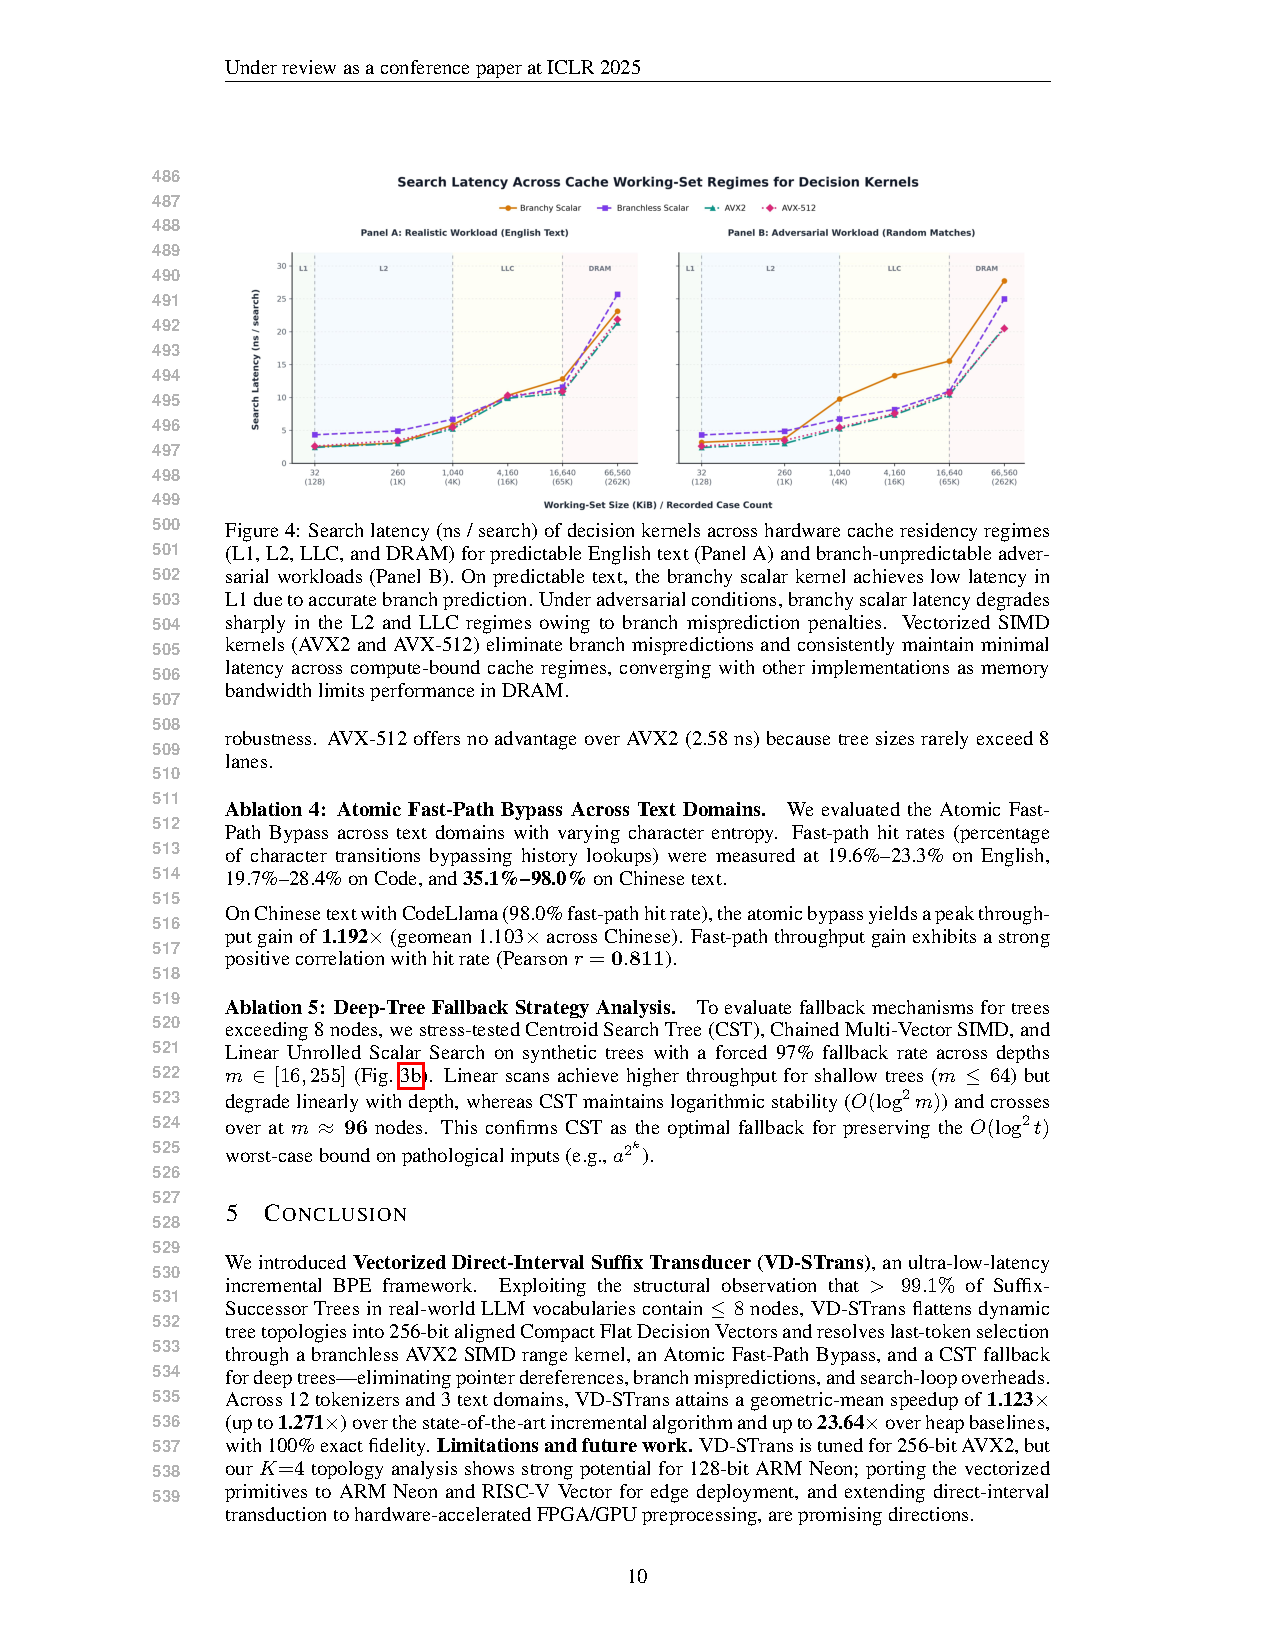
\includegraphics[width=0.2\textwidth]{figures/fig1_pdfs/page9.pdf}\\
    \hline
  \end{tabular}}
  \caption{\textbf{Case study.} \sname~independently establishes a novel approach that achieves a 10.9\% relative improvement over the human-designed state-of-the-art baseline~\citep{jiang2026incremental}. Moreover, evaluated under the ICLR peer-review procedures, this AI-authored paper is accepted, receiving impressive scores of 8.0 from ScholarPeer and 6.5 from the Stanford Agentic Reviewer.}
  \label{fig:qualitative_results}
\end{figure}

Scientific discovery has long been the hallmark of human ingenuity, defined by the ability to identify the boundaries of current knowledge and venture into the unknown. With the rapid advancement of foundation models \citep{team2023gemini, liu2024deepseek, singh2025openai}, artificial intelligence (AI) is transitioning from a passive conversational assistant to an active participant in the scientific process \citep{xu2025comprehensive, meng2026scientistone,jansen2025codescientist}. The ultimate ambition of this paradigm is purely \emph{problem-driven autonomous discovery}: a human researcher simply specifies a scientific challenge, and an autonomous AI independently navigates the landscape of human knowledge, diagnoses theoretical and empirical bottlenecks, formulates novel hypotheses, and executes the end-to-end research lifecycle on its own to pioneer the human knowledge frontier.

Despite recent progress in the field of autonomous research agents \citep{tang2026ai,weng2025deepscientist,yamada2025ai}, a substantial gap remains between automated assistant systems and rigorous empirical scientific standards. Existing systems primarily focus on optimizing single-scalar metrics on isolated benchmarks, lacking the multi-dimensional reasoning capabilities required to tackle complex scientific problems \citep{chen2026mars,jin2026toward}. More importantly, current agents lack the closed-loop empirical rigor of human scientists who continuously iterate based on evidence. They cannot systematically conduct ablation studies to isolate causal mechanisms for improvement, nor can they engage in dynamic peer-review processes essential for validating ideas and addressing methodological critiques through targeted supplementary experiments.

To overcome these fundamental challenges, we introduce \emph{\sname}, an expert-level autonomous multi-agent framework designed to pioneer the frontier of human knowledge (see Figure~\ref{fig:problem_setup}). Specifically, \sname~operates on a foundational division of labor: the human researcher defines the target scientific challenge, while the AI autonomously orchestrates the path to advance it. To rigorously demonstrate this capability against the highest standard of scientific rigor, we subject \sname~to the real-world testing ground: given competitive peer-reviewed human research from top-tier AI venues (e.g., ICLR, ICML, NeurIPS), \sname~must independently discover meaningful advancements beyond the established state-of-the-art, while simultaneously demonstrating that its autonomous scientific discovery process is measurable, reproducible, and transparent.

\begin{figure*}[t]
\centering
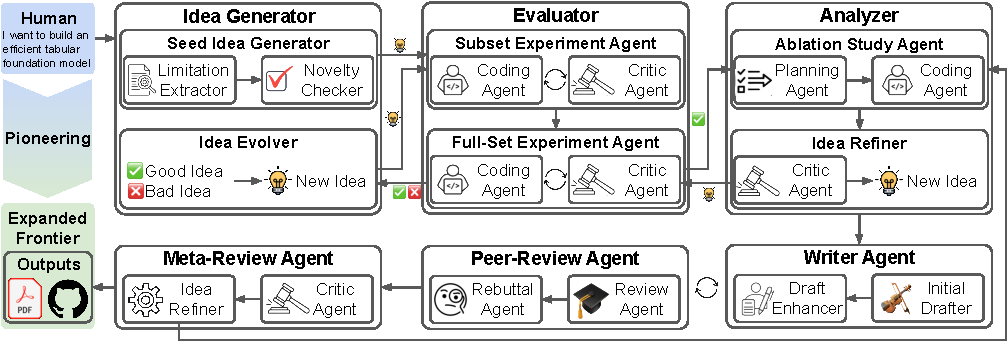
\includegraphics[width=\linewidth]{figures/scientisttwo_overview.pdf}
\caption{\textbf{Overview.} \sname~leverages previous experiments, ablation studies, and reviewer to generate and validate novel ideas that advance human state-of-the-art baselines, verifying each idea across multiple datasets and evaluation metrics. Additionally, it simulates the peer-review process to iteratively refine drafts into publication-ready papers.}
\label{fig:overview}
\end{figure*}
% \input{figures/coverage}
To achieve expert-level rigor across diverse disciplines demanded by top-tier science, \sname~coordinates a collaborative ecosystem of specialized agents (see Figure~\ref{fig:overview}):
\begin{itemize}
    \item \emph{Holistic Benchmark Reasoning \& Efficient Screening}: Rather than overfitting to a single metric, \sname~evaluates proposed ideas across comprehensive, multi-dataset benchmarks. To balance computation efficiency, it employs a subset-first evaluation strategy, rapidly filtering ideas on representative benchmark slices before allocating compute to full-scale experiments.
    \item \emph{Ablation-Driven Hypothesis Refinement}: Emulating the empirical rigor of expert researchers, \sname~autonomously designs and executes ablation studies to isolate individual component contributions, dynamically pruning ineffective components and refining its core hypothesis.
    \item \emph{Dynamic Peer-Review \& Rebuttal Loops}: To ensure publication-grade validity, generated drafts are critiqued by a simulated Peer-Review Agent. Rather than treating review comments as passive editorial guidance, a dedicated Rebuttal Agent actively conceives, codes, and executes targeted supplementary experiments to address critique. A Meta-Review Agent oversees this cycle, triggering recursive refinement loops until rigorous acceptance criteria are satisfied.
\end{itemize}

We evaluate \sname~across 107 diverse research challenges encompassing diverse areas such as optimization, reinforcement learning, large language models (LLMs), and theory (see Figure~\ref{fig:problem_setup}). Specifically, \sname~successfully advances 80.4\% of the target problems, delivering an average relative performance gain of 25.2\% over the original human state-of-the-art baselines. Furthermore, the autonomously generated manuscripts and executable codebases consistently achieve high acceptance rates across independent automated peer-review evaluations with high scores. These results demonstrate that \sname~moves beyond passive empirical problem-solving, serving as an autonomous pioneer capable of systematically expanding the frontiers of scientific knowledge.